\documentclass[12pt]{extarticle}
\date{}
\usepackage[clines,headsepline,autooneside,
automark,markuppercase]{scrpage2} 
\setheadsepline{1pt}
%\setfootsepline{0.4pt}
\ifoot{}\cfoot{\pagemark}\ofoot{}
\hfuzz=20pt
\vfuzz=20pt
\hbadness=2000
\vbadness=\maxdimen
\pagestyle{scrheadings} % use plain for standard
\usepackage{xcolor}
\usepackage[utf8]{inputenc}
\usepackage{cite}
\usepackage{graphicx} 	%package to include graphics
\usepackage{setspace} 	%package to set space between lines
\usepackage{lscape} 	%package to rotate pages
\usepackage{booktabs} 	%package for nice tables
\usepackage{amsmath,
amsfonts,amssymb}		%LateX mathformulas and typography
\usepackage{pifont}
\usepackage{listings}	%for code snippets
\usepackage{nomencl}
\makenomenclature
\usepackage{array}		%extends array and tabular environments
\usepackage{textcomp}	%package support of the text companion fonts
\usepackage{exscale}	%package for nice summation sign 
\usepackage{tabularx}	%package for column width and linebreaks in table cells
\usepackage{ragged2e}	%less raggedness commands \flushleft(right)
\usepackage{multirow}	%package to combine cells in tables
\usepackage{eurosym} 	%package to get eurosymbol per \euro
\usepackage{enumerate}	%package to make nice lists
\usepackage{ulem}		%package for uline
\usepackage{wasysym}	%package for weird symbols and geometric figs
\usepackage{hyperref}	%package for clickable TOC
\usepackage[title,
titletoc,toc]{appendix} %package for appendix
\usepackage{cleveref}
\usepackage[T1]{fontenc}
\usepackage{lmodern}
\usepackage{pdfpages}
\usepackage{color}
\usepackage{framed}
\usepackage{caption}
\usepackage{bbm}
\usepackage[section]{placeins}	%	places figures in their corresponding section
\setlength{\parindent}{4em}
\setlength{\parskip}{0.5em}
\setlength{\headheight}{1.1\baselineskip}

\definecolor{graycolor}{rgb}{.35,.35,.35}
\newenvironment{fshaded}{%
\def\FrameCommand{\fcolorbox{framecolor}{shadecolor}}%
\MakeFramed {\advance\hsize-\width \FrameRestore}}%
{\endMakeFramed}
\lstset{language=C++,
                basicstyle=\ttfamily,
                keywordstyle=\color{blue}\ttfamily,
                stringstyle=\color{red}\ttfamily,
                commentstyle=\color{green}\ttfamily,
                morecomment=[l][\color{magenta}]{\#},
                numbers=left,
                escapeinside={(*}{*)}
                }
\newcommand{\R}{\mathbb{R}}
\newcommand{\Ro}{\mathcal{R}}
\newcommand{\Sc}{\mathcal{S}}
\newcommand{\Tr}{\mathcal{T}}
\newcommand{\Mod}{\mathbb{M}}
\newcommand{\Pro}{\mathbb{P}}
\newcommand{\Vie}{\mathbb{V}}
\newcommand{\N}{\mathbb{N}}
\newcommand{\daf}{$\implies$}
\newcommand{\bs}{\backslash}
\newcommand{\Z}{\mathbb{Z}}
\newcommand{\Q}{\mathbb{Q}}
\newcommand{\lmin}{\lambda_{\mathrm{min}}}
\newcommand{\F}{\mathcal{F}}
\newcommand{\C}{\mathcal{C}}
\newcommand{\Rn}{\mathbb{R}^n}
\newcommand{\Linie}{\rule{\linewidth}{0.6mm}}

%Shortcut for table in the Evaluation
\newcommand{\rating}{\begin{tabular*}{0.85\textwidth}
{| p{\textwidth/4} | p{\textwidth/16} | p{\textwidth/16}
 | p{\textwidth/16} | p{\textwidth/4} |}\hline1 (totally disagree)
 &2&3&4&5 (totally agree)\\
\hline\end{tabular*}}
%Shortcut ends

\begin{document}
\begin{titlepage}
\newcommand{\HRule}{\rule{\linewidth}{0.5mm}}
\center
\textsc{\LARGE Universität zu Köln}\\[1.5cm]
\textsc{\Large Masterarbeit}\\[0.5cm] 
\textsc{\large 3D-Interaktion und Visualisierung
 in der Wissenschaft}\\[0.5cm] 
\HRule \\[0.4cm]
{ \Large \bfseries 
SAVKiT: Visualization and Multimodal Manipulation of Stereographic 3-D Objects}\\[0.4cm]
\HRule \\[1.5cm]
\begin{minipage}{0.4\textwidth}
\begin{flushleft} \large
\emph{Presented by:}\\
Pedro Fernando \\
Arizpe Gomez\\ 
\emph{Matrikelnummer:}\\
5500958 
\end{flushleft}
\end{minipage}
~
\begin{minipage}{0.4\textwidth}
\begin{flushright}
\large\emph{Professor:} \\
Prof. Dr. Lang
\large\emph{Supervisor:} \\
Dipl.-Inf. Daniel Wickeroth
\end{flushright}
\end{minipage}\\[4cm]
{\large 01.06.2016}\\[3cm] 
\vfill 
\end{titlepage}
\tableofcontents
\pagebreak{}
\printnomenclature
\section{Introduction} \label{sec:Int}
The main \textbf{purpose} of this project is to implement a user interface for the visualization of 3-D objects on a 55 inch-3-D capable screen with 1920x1080 resolution and 240Hz frame rate through a stereoscopic representation, and to enable their manipulation through the integration of the functionality of a multi-touch-overlay with unlimited touch point recognition and 200 fps sample rate and a camera with a 512×424 \nomenclature{CMOS}{Complementary Metal Oxide Silicon} 3D Time-of-Flight Image Sensor with Multi-Frequency Photo-Demodulation up to 130MHz and 2\nomenclature{GS/s}{Gigasamples per second} \nomenclature{ADC}{Analog to Digital Converter}.

Any hardware that complies with the above mentioned technical requirements would suffice for the purposes of this work. Therefore, the screen of choice for this specific project is a Samsung UN55F7500 smart 3-D-TV. The multi touch overlay is a G4 Series of PQlabs and the sensor is a Kinect 2.0 camera.

The aspiration of this work is to explore and investigate certain aspects of the human computer interaction (HCI) related to natural user interfaces (NUIs). Hence, the \textbf{hypothesis} presented by this project can be enunciated as follows:

\begin{quotation}
Modal redundancy is more precise, efficient and user friendly for artifact and scenario RST virtual object manipulation tasks than modal specialization on artifact and scenario respectively.
%Modal redundancy is more precise, efficient and user friendly for the virtual object manipulation tasks of rotating, scaling and translating (RST) of artifact and scenario than modal specialization on artifact and scenario respectively.
%Gesture redundancy across input methods is more efficient for object and scenario manipulation than modal specialization.
%It is better if the user can manipulate the object and the scenario with touchscreen and free hand movements than separating the scenario and object manipulation between these input modalities. 
\end{quotation}



%define gesture (scholar: gesture, position, signal)
\subsection{Definitions}
Due to the fact that throughout the literature not all definitions are uniform, the definition of some central concepts need to be specified for the specific purposes of this work.

\subsubsection {Multimodality}
In conformity with the definition proposed by Bourget \cite{multimodality} from the Queen Mary University of London, multimodal interaction refers to interaction with the virtual and physical environment through several natural modes of communication. In the particular case of this project, it refers specifically to touch and free hand gestures.

\subsubsection {Modal redundancy}
Two or more input modalities are redundant within a user interface (UI) when the same type of visualization manipulation can be carried out by any of them indistinctly.

\subsubsection {Modal specialization}
According to Laviola\cite{MSVTK} from the Brown University Site of the NSF Science and Technology Center for Computer Graphics and Scientific Visualization, a particular modality is specialized when it is always used for a specific task because it is more appropriate and/or natural for that task.\\

\subsubsection {Direct Manipulation:} Back in the 70\rq{}s, direct manipulation was understood as the possibility to interact \lq\lq{}directly\rq\rq{} with the windows on the screens using the mouse. Actions such as rotating, dragging and moving would be considered as direct manipulation.

In the 80\rq{}s, Ben Shneiderman from the University of Maryland \cite{DirManSh} cited display editors, primitive video games and even programming of industrial robots to replicate human actions as examples for direct manipulation.

Later on, as the first touch screens appeared, this concept evolved in meaning, redefined to be the interaction with objects \lq\lq{}directly\rq\rq{} underneath the fingers.

Considering this, the definition of direct manipulation used in this work is:
\begin{quotation}
An interaction between the user and the visualization that translates the movements of the first directly into an appropriate and proportional transformation of the second with immediate visual feedback.
\end{quotation}

\subsubsection {Visualization} Foley and Ribarsky suggest a definition of visualization that coincides with the connotation of this work: \cite{FoleyVisualization}

\begin{quotation}A useful definition of visualization might be the binding (or mapping) of data to a representation that can be perceived. The types of binding could be visual, auditory, tactile, etc. or a combination of these
\end{quotation}

\subsubsection {Gesture} In accordance to George and Blake, the definition of gesture referred to in this work is: \lq\lq{}Gestures are metaphors for discrete, indirect, intelligent interaction\rq\rq{} \cite{GestureDef}. More specifically, free hand gestures are defined as specific body positions and signals that can be interpreted by the hardware and translated into an information stream that triggers certain procedures within the simulation.
%Define position/signal?
\subsection{Organization}
The remainder of this paper is organized in the following
manner: Section \ref{sec:Soa} describes the related previous work, section \ref{sec:Mot} states the specific problematic and further explains the motivation for this project. Section \ref{sec:AV} describes the precursory software and provides some technical and theoretical framework and section \ref{sec:Sav} presents the new software. Section \ref{sec:Eval} and \ref{sec:Res} present the design and results of an expert survey, respectively. Finally, section \ref{sec:Con} presents the concluding remarks and asserts some possibilities for further work.

\section{State of the Art}\label{sec:Soa}
%++ related work: Was machen sie, warum ist das scheisse und warum ist meins besser
This section describes the current state of the science regarding stereoscopic 3-D visualization, manipulation and Natural User Interfaces (NUIs)

In his book \lq\lq{}A brave NUI World\rq\rq{}\cite{NUIWorld}, Wigdor makes a clear differentiation between the possibilities that specialized hardware can offer and the factual naturality of the interaction. He states that the hardware itself doesn\rq{}t define or guarantee a NUI, it just gives the opportunity to create one. 

Moreover, the characterization as NUI depends on the design of the interface and its capability of adapting and applying new technologies to utilize human capabilities and empiric experience to apply adequately to the given contexts and tasks.

This differentiation is very important when attempting to create a NUI, since the hardware is just a tool that allows for better gesture implementation, but the adequate application and the implementation of intuitive gestures that ensure a natural functionality is indispensable.

\subsection {Previous Theses}
This subsection describes the work previously done by other students who also implemented and explored multi-touch and free hand gesture interaction for virtual reality (VR).

\subsubsection {UTouch3D}
Baumesberger designed and implemented a self-designed multi-touch screen that can display 3-D virtual objects through stereoscopy. He called it uTouch3D\cite{Bau10,Deli13}.

The touchscreen of the uTouch3D can theoretically track an unlimited number of fingers simultaneously. This feature offers the user a further possibility of interaction with virtual objects. UTouch3D\rq{}s user interface exploits this possibility and allows the user to manipulate the visualization.

The original version of the program \cite{Bau10} is designed to allow the user to select, rotate, scale and translate the objects in the visualization through touch gestures. The user can switch between these interactions by changing the amount of fingers in the screen or the duration of contact of a single finger.

Despite its advantages, the uTouch3D also had a downside, since the touchscreen movements are still limited to a two dimensional plane and the displayed objects are in three dimensions, which makes it necessary to implement complex gestures to compensate the missing dimension.

Furthermore, the finger tracking mechanism encountered some difficulties regarding the thickness of every individual finger and continuity of the tracking, thus limiting the factual number of simultaneously detected fingers and restraining the theoretical functional possibilities.

Delisavas \cite{Deli13}enhanced the functionality of uTouch3D by incorporating free hand movements into the interface. These movements are read by a kinect camera 1.0. He modified the interface to accept touch, free hand and combinations of both inputs. He also exploited the hand tracking function of the camera to improve the tracking accuracy of the touch screen.

Nonetheless, the technical limitations of this camera narrowed the interaction possibilities. For example, that version of the camera could not yet quickly recognize if the hand was open or closed without excessive modifications and unreasonable computational effort (See \cite{HandRec})

\subsection {Omicron project and SAGE2}
The Omicron project is a software from the Electronic Visualization Laboratory of the University of Illinois in Chicago. It is currently implemented in the CAVE2 environment, which combines features of the first version of the CAVE; a multiwall, stereoscopic visualization\rq{}s environment; and tiled display walls (TDW).

Omicron can receive data from several input types, including touch overlays and motion tracking system. It is specially interesting because the touch overlays interface is based on the same touchscreen hardware as the project of this work, namely PQLabs Touchscreen.

This software specializes in the integration of several input devices. Then it streams data from these heterogeneous devices in such a manner that the SAGE2 server can interpret\cite{SAGE2}. The software described in this work contains modules that serve this same purpose. Both projects allow the user to decide on his method of input, and hereby they offer more possibilities of interaction.

However, the SAGE2 project focuses rather on the web-based collaboration than the visualization and manipulation of objects.

\subsection {Kinoogle}\label{subsec: kinoogle}
Kinoogle\cite{Kinoogle} is a natural interaction interface for Google Earth using Microsoft Kinect. It allows the user to control google earth through hand and full body gestures.\footnote{As this Kinoogle paper was written, only Kinect 1 camera was available in the market, therefore, the hand state function was not fully available} The user can pan, zoom, rotate, tilt and jump to street view by using predefined body gestures that are conceptually similar to the gestures used by this project\rq{}s software. (see subsection \ref{KinectGestures})

\subsection {Other software}
The development of new software and hardware for 3-D object visualization and manipulation has been recently boosted by the appearance of head mounted devices (HMDs), like Oculus-Rift as an example for submersive virtual reality or Google Glasses and HoloLens for hybrid reality.

Fluke and Barnes\rq{} (2016)\cite{NASA} paper, from the SAO/NASA Astrophysics Data System, regarding the ultimate display, ponders whether 3-D data visualization in immersive stereoscopic virtual reality in form of the CAVE2 or the Oculus-Rift would help astronomers to better process captured data.

However, they conclude by acknowledging the flaws and shortcomings of both:
\begin{quotation}
As a low-cost, highly portable solution, HMDs remain an intriguing option. From the perspective of display quality, HMDs clearly have a long way to go before they match either the visual acuity or binocular disparity limit. It seems very unlikely that there will be orders of magnitude changes here in the short term.

A CAVE2 configuration can reach the visual acuity limit and fill the horizontal FOV, but does not fare quite so well with vertical coverage. \cite{NASA}
\end{quotation}

\section{Motivation and Problem Statement}\label{sec:Mot}
%TODO: complement with State of the art, be more concrete
\subsection{Motivation}
This section explains the motivation behind this project. As early as 1988, computer scientists recognized the importance of simple direct manipulation controllers. Chen et al.(1988) also outlined some application possibilities:
\begin{quotation}
\lq\lq{}Currently, simple direct manipulation controllers do not exist for 3-D object positioning. The design of such controllers could be important interface contributions for application environments such as manufacturing, architecture, and engineering design, which rely heavily on the display and control of three dimensions.\rq\rq{} \cite{3DOn2D88}
\end{quotation}

This statement elucidates the importance of the creation of newfangled input methods or even user interface concepts. These should give the user the feeling of continuity between his empiric experience of object manipulation and his interaction with the virtual objects. These characteristics equate those of a NUI.

In Wigdor\rq{}s words, \cite{NUIWorld} Users naturally develop associations between what they want to do and where they do it from memory-triggered context. This delineates the core of the problem statement.

The essence of this project lies in the challenge of expanding the user\rq{}s real world experience to the manipulation of virtual objects through natural movements. Notwithstanding that industry standards dictate most design canons for user interfaces, the pursuit of neoteric intuitive interaction possibilities is still worthwhile.

%purpose: public display-> museums-> natural interaction metaphores
%TODO: Analysis of scenario, one object. requirements for interaction technique.
\subsection{Problem Statement}
Virtual three-dimensional objects originating from design or 3-D scans are becoming increasingly common. As stated by Yuan et al. \cite{3DTV}, \lq\lq{}The recent proliferation of stereoscopic three dimensional (3D) video technology has fostered a large body of research into 3D video capture, production, compression and delivery. However, little research has been dedicated to the design practices of stereoscopic 3D video interaction\rq\rq{}. Therefore, a need for adequate visualization manipulation possibilities has emerged.

The specific purpose of this project is the design of a software that can cope with these visualization manipulation necessities taking advantage of several input possibilities.

The concrete target scenario of this project is the visualization of a single virtual object.

The main utilization potentiality of this project is the public display in museums and similar interaction environments, where the public can get a better and more interactive visualization experience.

Another utilization opportunity is found on the didactic. Educational facilities could use this software as a tool for interactive learning, offering pupils an enhanced learning process.

For example, this software can display anatomically correct organs as a stereogram, which would help life sciences students to assimilate better the visual information and expedite the learning process. As opposed to 2-d schemes and pictures, stereograms provide a sense of depth and the possibility to observe the object from all angles.

For diagnosis purposes, this program could also be a great supporting tool for medical professionals, allowing for an effective and non invasive method of analysis.

\subsection{MoSCoW}
The functional requirements set for this project can be categorized according to the MoSCoW \cite{Moscow} prioritization method. This method suggests a differentiation between what the program must, should, could and won\rq{}t do.

There has been some criticism regarding this technique, due to its lack of precision concerning the guidelines for categorization. Wiegers \cite{Wiegers} states that this method lacks analysis of importance and urgency. However, for the purposes of this work, the consideration of forthcoming releases or a development time-box is unimportant, and therefore MoSCoW remains a suitable method.

Naturally, most of the requirements for this software have been inherited from Laurentius work \cite{AV}

\subsubsection{What must the program do?}
\begin{enumerate}
\item
The program \textbf{must} be able to display a 3-D virtual object through stereoscopy.
\item
The program \textbf{must} be able to interpret 3-D scans in form of polygon and stereolitography file types.
\item
The program \textbf{must} accept three different types of input: mouse/keyboard, touchscreen and free hand movements.
\item
The user, using any of the three input methods \textbf{must} be able to rotate the displayed object and the camera in all directions, giving 3 DOF for rotation.
\item
The user, using any of the three input methods \textbf{must} be able to translate the displayed object in all directions, giving 3 DOF for translation.
\item
The visualization \textbf{must} be in perspective mode.
\item
The program \textbf{must} display a real-time visual feedback for all manipulation interactions.
%\item
%The program \textbf{must} give the option to display the object with or without color information from PLY files.
%\item
%The program \textbf{must} provide lighting by four spot lights whose intensity and position can be adjusted in all three spatial axes to generate the desired shadows, which are necessary for optimal visibility of the details of the object.
%\item
%The program \textbf{must} allow the user to save the view configuration of the object. This concerns in particular the rotation of the object and the camera; the zoom factor; the orientation and parameters of the lamps.
%\item
%The program \textbf{must} allow the user to rotate the camera exactly by one degree with special buttons to enable the capture of the usual 6-fold view (front, rear, left, right, up, down) for scientific publications.
\item
The software \textbf{must} be open source and the source code must be made accessible and can be changed, which is ensured by its own license, but also by that of the included libraries.
\item
The code \textbf{must} be sufficiently commented to allow future expansion by any other programmers.
\end{enumerate}

\subsubsection{What should the program do?}
\begin{enumerate}
%\item
%The program \textbf{should} be able to display the width, height and thickness of the object in millimeters.
%\item
%The program \textbf{should} give the user the option to display overlapping layers of the object with additional information. For example, automatically detected edges or depressions of the object.
%\item
%The program \textbf{should} give the option to tack a note at any point on the surface of the displayed object. Its textual content stands on the left edge of the window and a line connects the note to the point on the surface to which the annotation is associated.
%\item
%The program \textbf{should} give the option to display or hide any note texts, if any exist.
\item
The program \textbf{should} be able to store the contents of the 3D display area as an image file at all times (Screenshot).
\end{enumerate}

\subsubsection{What could the program do?}
\begin{enumerate}
\item
The program \textbf{could} include gestures that isolate interaction types, for example, the user could scale the object with a specific gesture.
\item
The program \textbf{could} include a status bar to report the current state of interaction to the user.
\end{enumerate}

\subsubsection{What won\rq{}t the program do?}
\begin{enumerate}
\item
The program \textbf{won\rq{}t} include gestures that require a combination of input types.
\item
The program \textbf{won\rq{}t} read nor save the current position of the table.
\item
The user \textbf{won\rq{}t} receive tactile feedback.
\item
The program \textbf{won\rq{}t} include tracking for wearable pointers.
\item
The program \textbf{won\rq{}t} offer the possibility to alter the object\rq{}s nodes nor edges.
\end{enumerate}

The implementation of gestures that combine several input types has been excluded to maintain the smoothness of the simulation and to avoid tracking inconsistencies between input devices. The position of the table and the referencing of hand and body positions relative to it has been intentionally left out to reduce error proneness and to allow the user to start the interaction anywhere.

\section{Technical background and primordial software}\label{sec:AV}
\subsection {Geometry and 3-D visualization}\label{subsec: geo}
The typical human-computer-interaction takes place through 2-D displays, therefore an optical illusion is necessary in order to visualize 3-D virtual objects and give the impression of depth. This illusion is called a stereogram.

\subsubsection {OpenGL}\label{subsec{OGL}}
Monitors and projectors can only display a finite number of picture elements (pixels) per frame. Therefore, many homogeneous transformation, projection and clipping operations are necessary to enhance the visualization experience. Hereby, a graphics library becomes an essential tool for visualization.

OpenGL enables a simplified implementation that includes all the necessary mechanisms to deal with geometry; through a visualization frustum, stereoscopy i.e. stereopsis, projection, perspective, coloring, opaqueness, shading, and buffering; in the form of predefined concepts, operations and variables inside a graphics library.

\subsubsection {Homogeneous transformations}\label{subsubsec Hom}
Let $\Mod\in \R ^{4\times 4}$ be the Model Transformation Matrix. This Matrix is a homogeneous matrix that contains all executed transformations of the visualized object. namely all $\Ro \in \R ^{4\times 4}$ for rotation matrices, $\Sc \in \R ^{4\times 4}$ for scaling matrices and $\Tr \in \R ^{4\times 4}$ for translation matrices. For the purposes of this project, $\Mod$ will be called the Artifact Matrix.\cite{RST}

Now let $\Vie\in \R ^{4\times 4}$ be the View Matrix. This Matrix is also a homogeneous matrix that maps all the world coordinates obtained by the previous transformation to camera coordinates.

Finally, let $\Pro\in \R ^{4\times 4}$ be the Projection Matrix. Since the main purpose of this project is to visualize objects and not to realize measurements, the most suitable choice for $\Pro$ is a perspective transformation.

The successive multiplication of $\Mod, \Vie$ and $\Pro$ results on the MVP matrix, which can be processed very efficiently by the graphic processing unit (GPU) giving room to a smooth and continuous visualization throughout the interaction.

\subsection{Artifact Viewer}
This subsection describes the original structure, functionality and form of the Artifact Viewer program (AV) which was the primordial\footnote{Primordial: That constitutes the origin or starting point from which something else is derived or developed, or on which something else depends; fundamental, basic; elemental.\cite{OED}} software of this project\cite{AV}. The AV is a visualization software that can read polygon (PLY) and STereoLithography (STL) files. The objects were displayed inside a Qt-based GUI on a monochromatic or color gradient background.

The original conception of the Artifact viewer was done with the purpose of devising a tool that could display archaeological objects in 3-D and give users the opportunity to manipulate several aspects of the visualization and also carry out measurements and annotations.

However, this program still maps the object into a two-dimensional representation and the input possibilities were limited to keyboard and mouse.

On the side bar the user has the possibility to interact with the configuration of the visualization and some mouse and keyboard events allowed further manipulation of the object.
\subsection {Structure and Functions}
	\subsubsection { File compatibility}
	AV is able to read from two types of files, *.stl and *.ply. This is managed by two plugins that can interpret the data on the files and transform it into an object.
	\subsubsection { Menu}
	The top screen menu offers pre-programmed tasks in four categories: file, tools, options and help.
	The \textbf{file} menu includes the options to open a new object in the visualization area and to save the current configuration of the visualization into an XML file.
	The \textbf{tools} menu included only the option to make a screen-shot of the current state of the visualization.
	In the \textbf{options} menu, the user can change the background color and, in case the vertex colors usage is deactivated, the user can select a color for the artifact.
	In the \textbf{help} menu, the about button offers information about the current version and the author, and the help button opens the documentation of the program.
	\subsubsection { 3-D Visualization panel}
	The visualization panel is the main part of the widget. Whenever a file is open, the virtual object is displayed.
	\subsubsection { Lighting}
	On the side menu, the user has the possibility to configure the lighting of the object. The shading model is based on \lq\lq{}Blinn-Phong shading\rq\rq{}. First of all, the first check box on the top left of this section, \lq\lq{}use lightning\rq\rq{} toggles the activation of lightning. The second one: \lq\lq{}lights visible\rq\rq{}, on the top right, toggles the visibility of of the lights ant the rotation circumference of the selected light. The program has four light sources that can be rotated around the object along these two circumferences. 
	
	If \lq\lq{}lights visible\rq\rq{} is on, lights are displayed as small lamps in pyramid form. The drop-down menu under the \lq\lq{}lights\rq\rq{} title is used to select one of the four lights and enable its rotation and intensity and distance modifications.
	\subsubsection { Rotation}
	The next item on the sidebar allows the user to make a controlled rotation of the camera by the selected amount of degrees in the selected direction (up, down, left, right) or of the artifact, clockwise or counterclockwise.
	\subsubsection { Visual Enhancements}
	The visualization can be modified, independently from lighting, to darken or brighten edges and to darken valleys.
	\subsubsection { Annotations and Points}
	The user can select a point in the surface of the object and create an annotation, if there are two selected points, he can measure the distance between these points. If exactly three points are selected, the program can measure the angle between the line connecting the first and second point and the line connecting the second and third points.
	If three or more points are selected, the program offers the possibility to calculate the convex surface connecting these points.
	\subsubsection { Mouse and Keyboard event handling}
	The AV can receive mouse, keyboard and combined input, for example if the shift key is pressed, the user can move the position of the camera by clicking and dragging the mouse. Without the shift key modification, the left mouse click is used for points and annotations and the right one to rotate the object.
	\subsubsection { Keyboard shortcuts}
	Some keyboard shortcuts are implemented to facilitate manipulations like toggling lighting and rotating
	
\section{SAVKiT}\label{sec:Sav}
%Unbedingt noch: Umfrage zu Bewegungen
This section describes the ideological conception of the program and presents the modifications from the original AV program that lead to the Stereoscopic Artifact Viewer with Kinect and Touch (SAVKiT).

\subsection {Concept}
The main idea behind SAVKiT is the implementation of a NUI that allows the user to execute all homogeneous manipulations described in \ref{subsubsec Hom}, namely rotation, scaling and translating through several input methods, allowing the user to choose the most adequate for his intention.

A very important characteristic of NUI is the intuitiveness of the movements. On touch screens, some movements have pushed through as industry standards, like pinch to shrink and split to enlarge. However, 3-D direct manipulation is still developing. Therefore, gestures and movements are also still maturing. Nevertheless, the movements and free hand manipulation possibilities considered in this project seem to be in accordance to other previous works, like Kinoogle \cite{Kinoogle}, as mentioned in subsection \ref{subsec: kinoogle}.

The program is designed to give the user the impression of being able to grab the object in the air and manipulate it in different ways, allowing for an intuitive translation of movements into visual feedback.

\subsection {Stereoscopy Implementation}
The first modification of the original program was the use of Quad-buffering to enable active stereoscopic display of the visualized objects (See \ref{app:StereoFormat}). For this purpose, the introduction of parallax, achieved through a second camera, was necessary, which also implied the duplication of all homogeneous transformations and projections.

\subsection {New Keyboard Shortcuts}
According to Shneiderman\rq{}s 8 golden rules \cite{Shneiderman}, designers should cater to universal usability, allowing frequent users to expedite routine tasks and have better control over the interface.
\begin{center}

\begin{tabular}{|c|c|} \hline
\textbf{Key Combination} & \textbf{Action}\\ \hline
Ctrl+O & Open File\\\hline
Ctrl+S & Save File\\\hline
Ctrl+F & Toggle Full-screen \footnote{This function is also available on the top screen menu} \\\hline
Ctrl+P & Screenshot\\\hline
Ctrl+M & Show Mouse\\\hline
Ctrl+H & Hide Mouse\\\hline

\end{tabular}
\end{center}


\subsection {Touch Screen Enhancements}

\subsubsection {Smart 3-D-TV Touchscreen Gestures}
This subsection contains the gestures that AV can interpret from the touchscreen. The kind of manipulation depends on the number of fingers on the screen. 

When a first finger touches the screen, the touchscreen coordinates are mapped to the widget coordinates where the object is displayed. If the mapped coordinates are inside of the widget, the touchscreen interaction begins. Successive fingers activate other functions, and if a finger leaves the screen, the interaction adapts to the new quantity of fingers on the touch screen. If no fingers are left, the touch screen interaction comes to an end.

\subsubsection* {One finger interaction}
If there is only one finger on the screen, then the user can change the position of the camera along the X and Y axes, giving the impression that the whole scenario is moving in the same direction as the finger on the screen.

Let $F_{1,t}=\begin{pmatrix} x_{1,t}\\y_{1,t}\\ \end{pmatrix} \in \R^2, t\in \Z$ be the initial finger position at frame t with $(x,y)$ coordinates $(x_{1,t},y_{1,t})$ and let $$\Delta F_{1,t}=\begin{pmatrix} \Delta x_{1,t}\\\Delta y_{1,t}\\ \end{pmatrix}=\begin{pmatrix} x_{1,t}-x_{1,t-1}\\y_{1,t}-y_{1,t-1}\\ \end{pmatrix}$$ be the finger displacement. Now let $\mathcal Oc_t$ be the origin of the camera at frame $t$. Then, the movement of the camera is calculated by:
$$\mathcal Oc_{t+1}=\mathcal Oc_t+\begin{pmatrix}\frac{-\Delta x }{6.3}\times\frac {CDO}{150}\\\frac{\Delta y }{6.3}\times\frac {CDTO}{150}\end{pmatrix}$$
where CDO is the distance from the current camera position to the origin.

\subsubsection* {Two-finger interactions}
If there are two fingers on the screen and the distance between them is increased, then the camera goes closer to the object, if the distance is reduced, then the camera goes further from the object, giving the impression of zooming in and out, respectively. If the line between the fingers is rotated, the object will rotate around the axis that is orthogonal to the screen plane.

Let $F_{i,t}=\begin{pmatrix} x_{i,t}\\y_{i,t}\\ \end{pmatrix} \in \R^2, t\in \Z$ be the position of finger $i$ at frame t with $(x,y)$ coordinates $(x_{i,t},y_{i,t})$. The distance between fingers at frame t $d_{t{{1,2}}}$ is calculated as follows:
$$d_{t_{1,2}}=\|F_{1,t}-F_{2,t}\|_1$$
where $\|\cdot \|_1$ is the $l_1$ norm, since its calculation is significantly more efficient than the euclidean distance. Then, the zooming operations are executed by the following formula:
$$CDO_t=CDO_{t-1}\cdot \frac{d_{t-1_{1,2}}}{d_{t_{1,2}}}$$
Now let $\overrightarrow{v_t}=F_{2,t}-F_{1,t}$ be the line between fingers at frame t. Then, the angle of rotation $\theta_{touch}\in [0,360]$ around the z axis is calculated by: 
\[\theta_{touch}\frac{-180}{\pi}\cdot \arccos(<\overrightarrow{u}, \overrightarrow{v}>)\]
\subsubsection* {Three-and-more-finger interaction}
If there are three or more fingers on the screen and they are moving in the same direction, a simulation of the trackball movement is initialized. Depending on the mode set for the trackball, the object follows a 3-D rotation as a sphere or in the plane. The speed of the trackball movement is divided by the number of fingers on the screen.

Let $F_{i,t}$ be defined as above. Let n be the number of fingers touching the screen, then the position of the pointer of the trackball movement is determined by:
$$\sum_{i=1}^n \frac{1}{n}F_{i,t}$$

\subsection {Kinect 2 Camera Gesture implementation}\label{KinectGestures}
Most current video games and applications for Kinect generate a pointer as an interaction dummy for the virtual world. SAVKiT uses relative position data, which means that the user can start interaction anywhere in the kinect camera space and the movement will be calculated from the relative position of the hands from frame to frame.

The program receives the coordinates of the hand position given by the kinect camera and transforms them to fit the visualization coordinates\rq{} orientation. Since the screen is used in an horizontal position, the following transformation is required:
$$\begin{array}{c}
\mathcal F: \R^3\to R^3; \\
\mathcal F:\begin{pmatrix} x\\y\\z\end{pmatrix}\mapsto \begin{pmatrix} x\\-z\\y\end{pmatrix}\end{array}$$
where $\mathcal F$ is applied to all coordinates received from the kinect camera in order for them to match the coordinates on the visualization environment.

The Kinect Camera 2.0 has the capability of recognizing the state of the hands. It can differentiate between a closed, open and lasso positions. (see Figure \ref{fig: OCL}).
\begin{figure}[ht!]
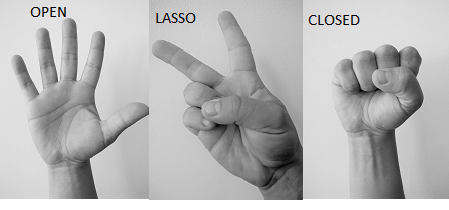
\includegraphics[scale=1.5]{Images/KinectHandStates.png}
\caption{Kinect Hand States depiction}
\label{fig: OCL}
\end{figure}\\
In their Microsoft Kinect natural user interface for Google Earth navigation, Boulos et al. \cite{Kinoogle} distribute the three visualization manipulation possibilities; namely rotate, scale and translate (RST); among two free hand gestures. Rotate and scale are executed with two closed hands and translation (pan) is done with one hand open and the other one closed. The interaction design of this project follows this example and extends it to isolate the scaling interaction into a third hand state, i.e. lasso, and offers two possibilities for translation.

In addition, the attempts to implement all three visualization manipulations into one gesture resulted in an unstable interaction with faulty visual feedback and great error susceptibility, despite the utilization of a Kalman filter.

Kinect interaction can be activated by holding both hands open for two seconds. Once the interaction is initialized, the following manipulations are possible:

\subsubsection {Rotate}\label{subsubsec Rot}
Both hands closed start the rotation, until one or both hands are opened. The rotation is programmed with 6 degrees of freedom (DOF).

The angle of the rotation is calculated by creating a vector between the point coordinates of both hands and then comparing its angle with the vector of the next frame by means of a dot product.

Let $R_t\in \R^3$ represent the coordinates of the right hand at frame $t, t\in \Z$ and $L_t\in\R^3$ represent the coordinates of the left hand at frame $t$. Then, the \textbf{angle of rotation }$\theta_{kinect}\in [0, 360]$ in degrees is given by:
\[\theta_{kinect}=\frac{180}{\pi}\cdot \arccos(<\overrightarrow{u}, \overrightarrow{v}>)\]
And the \textbf{axis of rotation} by
\[Axis=\overrightarrow{u}\times \overrightarrow{v}\]
where $$\overrightarrow{u}=\frac{R_{t-1}-L_{t-1}}{\|R_{t-1}-L_{t-1}\|}\ , \ \overrightarrow{v}=\frac{R_t-L_t}{\|R_t-L_t\|}$$.
At frame $t=0$ the initial positions of the hands are captured, therefore these formulas are valid for $t\geq 1$.

To ensure a smooth interaction, all rotations with an angle of more than 30 degrees are ignored. Furthermore, the axis of rotation remains befitting to the visualization axes, meaning that previous rotations of the artifact matrix do not interfere with the direction of rotation. (see Appendix \ref{app:codeRot}, line \ref{lineDerotate})

\subsubsection {Scale}\label{subsubsec Scale} If both hands have two fingers up, recognized as lasso position by the kinect, the program initializes the scaling mode. The artifact can be proportionally scaled by changing the separation between hands while keeping the hand position.

Let $R_t$ and $L_t$ be defined as in \ref{subsubsec Rot}. Then, let $D_t$ be the separation between the hands at frame $t$, defined by $D_t=R_{t}-L_{t}$. Herewith, the scaling factor $s_t\in \R$ between frames is calculated by:
$$s_t=\frac{D_{t-1}}{D_t}, t\geq 1$$
Once again, to ensure the smoothness of the rotation and to avoid abrupt changes, scaling factors outside of the tolerance borders are ignored, meaning that only if $0.75<s_t<1.5$, the scaling takes place.


\subsubsection {Translate} \label{subsubsec: Translate} The left hand up and open with the right one closed starts a homogeneous translation of the model matrix, whereas the right hand\rq{}s change of position determines the translation of the artifact, and the left one works as the \lq\lq{}signal\rq\rq{}, meaning that the movement stays on as long as the left hand remains open, or until the right hand opens

Let $R_t$ and $L_t$ be once again defined as above. The translation vector $\Delta_r\in \R^3$ applied to the Artifact Matrix is determined by:
$$\Delta_r=R_{t-1}-R_t, t\geq 1$$
Anew, all previous rotations of the Artifact Matrix are ignored to guarantee an intuitive interaction. The object moves always in the same direction as the hand of the user.

The right hand up and open, the left one closed starts a homogeneous translation of the projection matrix, where the left hand\rq{}s change of position determines the translation of the projection, and the left one works as the \lq\lq{}signal\rq\rq{}, meaning that the movement stays on as long as the right hand remains open, or until the left hand opens.

The translation vector $\Delta_l\in \R^3$ applied to the projection Matrix is determined by:
$$\Delta_l=L_{t-1}-L_t, t\geq 1$$

Similar to the model translation, the projection follows the movement direction of the hand.
\subsubsection {Untracked or unknown states} If the position of both hands has not been tracked for 5 seconds or if the state of the hand has been unknown for 10 seconds, then the interaction with the kinect camera stops.\footnote{unknown and \lq\lq{}not Tracked\rq\rq{} states just report approximate coordinates} 

\section{Evaluation} \label{sec:Eval}
The evaluation of this project was in form of a consultation and survey of 10 experts to assess the functionality, usability and intuitiveness of the program. A template of this survey can be found on Appendix \ref{app:survey}\cite{QDsus}

\section{Results}\label{sec:Res}
This section presents the results of the previously mentioned survey.

\section{Concluding Remarks and future work}\label{sec:Con}
This section includes a small summary of the thesis, states adequate conclusions and suggests possibilities for further investigation of the topic.
\bibliography{MasterRef}
\bibliographystyle{ieeetr}
\pagebreak
\begin{appendices}
\section{code}
\subsection {Stereo format Code}\label{app:StereoFormat}
\begin{lstlisting}
QGLFormat stereoFormat;
stereoFormat.setSampleBuffers(true);
stereoFormat.setStereo(true);
this->setFormat(stereoFormat);
\end{lstlisting}
\subsection {Kinect Rotation Code}\label{app:codeRot}
\begin{lstlisting}
//refresh hand positions
 if(!mano.isLeft)
 {
 m_kNewRightRotPos=QVector3D((qreal)mano.x,
 (qreal)-mano.z,(qreal)mano.y);
 }
 if(mano.isLeft)
 {
 m_kNewLeftRotPos=QVector3D((qreal)mano.x
 ,(qreal)-mano.z,(qreal)mano.y);
 }
 //draw new rotation line
 m_kNewRotVec=m_kNewRightRotPos-m_kNewLeftRotPos;
 //get angle
 m_KRotAngle=acos(QVector3D::dotProduct(
 m_kOldRotVec.normalized(),m_kNewRotVec.normalized()
 ) )* 180.0f / PI
 //get axis
 m_axis = QVector3D::crossProduct(m_kOldRotVec.normalized(),
 m_kNewRotVec.normalized());
// get ScaleFactor
m_kScFactor=m_kNewRotVec.length()/m_kOldRotVec.length();
 //rotate by axis and angle
 if(m_KRotAngle< 30 | | m_KRotAngle>330)
 {
m_MatrixArtefact.translate(m_model->m_centerPoint);
m_MatrixArtefact.translate(m_camOrigin);
m_axis = m_MatrixArtefact.inverted().mapVector(m_axis)(*\label{lineDerotate}*)
m_MatrixArtefact.rotate(m_KRotAngle,m_axis.normalized());
m_MatrixArtefact.scale(m_kScFactor);
m_MatrixArtefact.translate(-m_camOrigin);
m_MatrixArtefact.translate(-m_model->m_centerPoint);
 }

 updateGL();
 //update hand positions and connection vector
 m_kOldLeftRotPos=m_kNewLeftRotPos;
 m_kOldRightRotPos=m_kNewRightRotPos;
 m_kOldRotVec=m_kNewRotVec;
\end{lstlisting}

\pagebreak{}
\section{Expert survey template}\label{app:survey}
\begin{center}
Gender:M/F\ \ \ Age:\_\_\_ Occupation (Major for students):\_\_\_\_\_\_\_\_\_\_
\begin{enumerate}
\item I think that I would like to use this system frequently

\rating
\item I found the system unnecessarily complex

\rating
\item I thought the system was easy to use

\rating
\item I think that I would need the support of a technical person to be able to use this system

\rating
\item I found the various functions in this system were well integrated

\rating
\item I thought there was too much inconsistency in this system

\rating
\item I would imagine that most people would learn to use this system very quickly

\rating
\item I found the system very cumbersome to use

\rating
\item I felt very confident using the system

\rating
\item I needed to learn a lot of things before I could get going with this system

\rating
\end{enumerate}
\end{center}
Thank you very much for your input.
\pagebreak{}
\section{Survey Handout}\label{app:Handout}
\setcounter{figure}{0}
\makeatletter 
\renewcommand{\thefigure}{HO. \@arabic\c@figure}
\makeatother
\begin{center}\begin{Huge}
SAVKiT: Stereographic Artifact Viewer with Kinect and Touch
\end{Huge}\end{center}
\subsection{Touchscreen}
\emph{One finger} on the screen moves the whole scenario. 
See figure \ref{fig: AT1F}.

\begin{center}
\begin{figure}[!h]
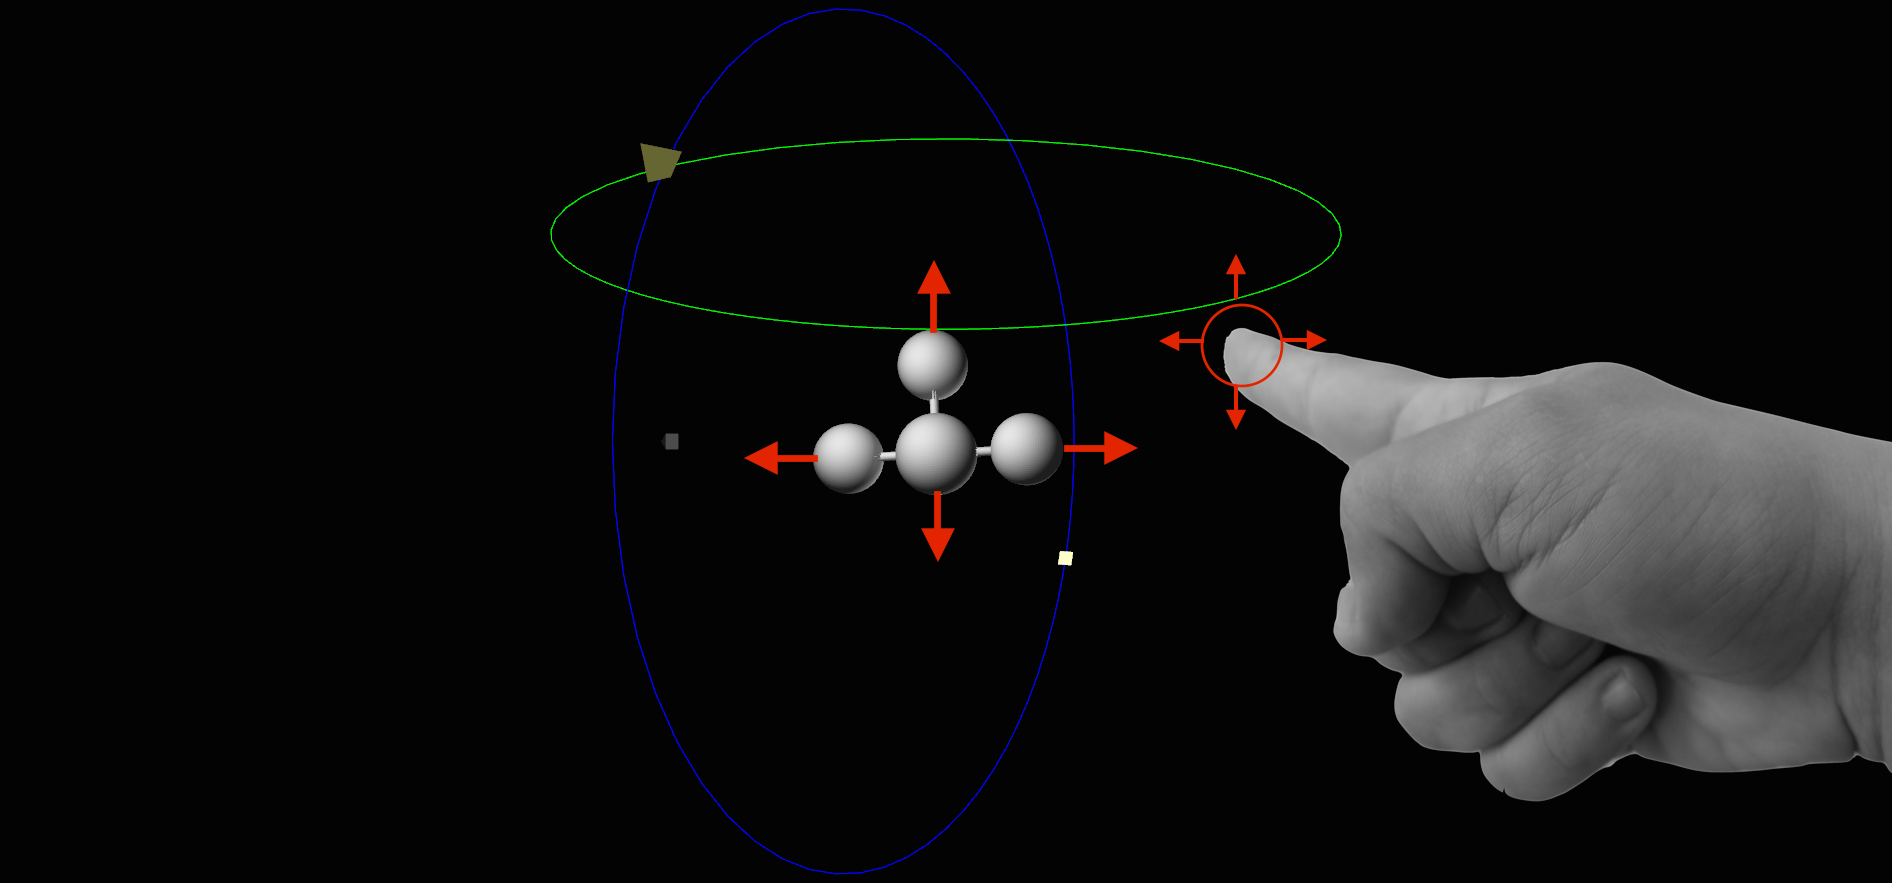
\includegraphics[scale=0.4]{Images/Touch1Finger.png}
\caption{One Finger Touch Interaction}
\label{fig: AT1F}
\end{figure}
\end{center}

\emph{Two fingers} on the screen activate zooming and rotation around the z-axis. both work simultaneously. Pinch to zoom and turn to rotate.
See figure \ref{fig: AT2F}.
\begin{center}
\begin{figure}[!ht]
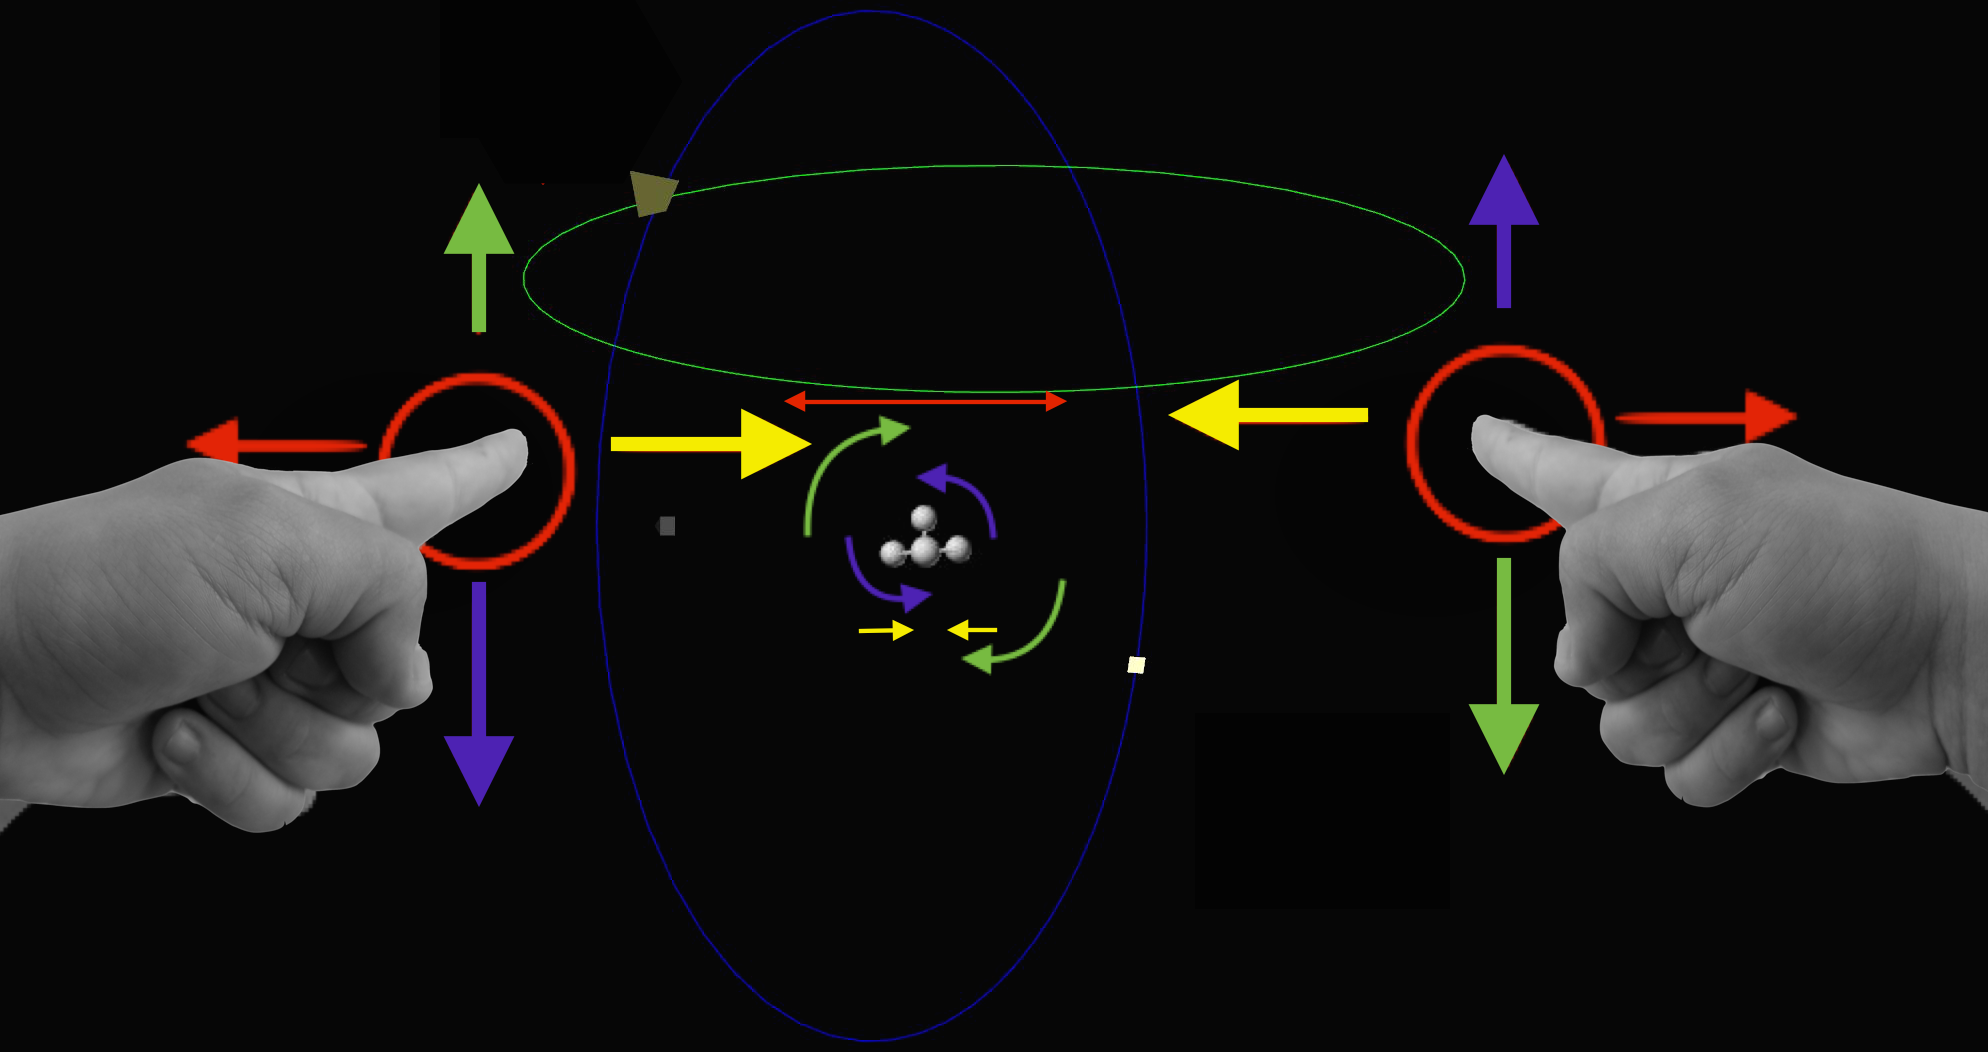
\includegraphics[scale=0.4]{Images/Touch2Fingers.png}
\caption{Two Finger Touch Interaction}
\label{fig: AT2F}
\end{figure}
\end{center}

\emph{Three} or more fingers on the screen rotate the object in 3-D around its center. The 3-D rotation creates a line between the geometrical center position of all fingers and the object\rq{}s center and rotates the object accordingly. The speed of the trackball movement is divided by the number of fingers on the screen.
See figure \ref{fig: AT3F}.
\begin{center}
\begin{figure}[!h]
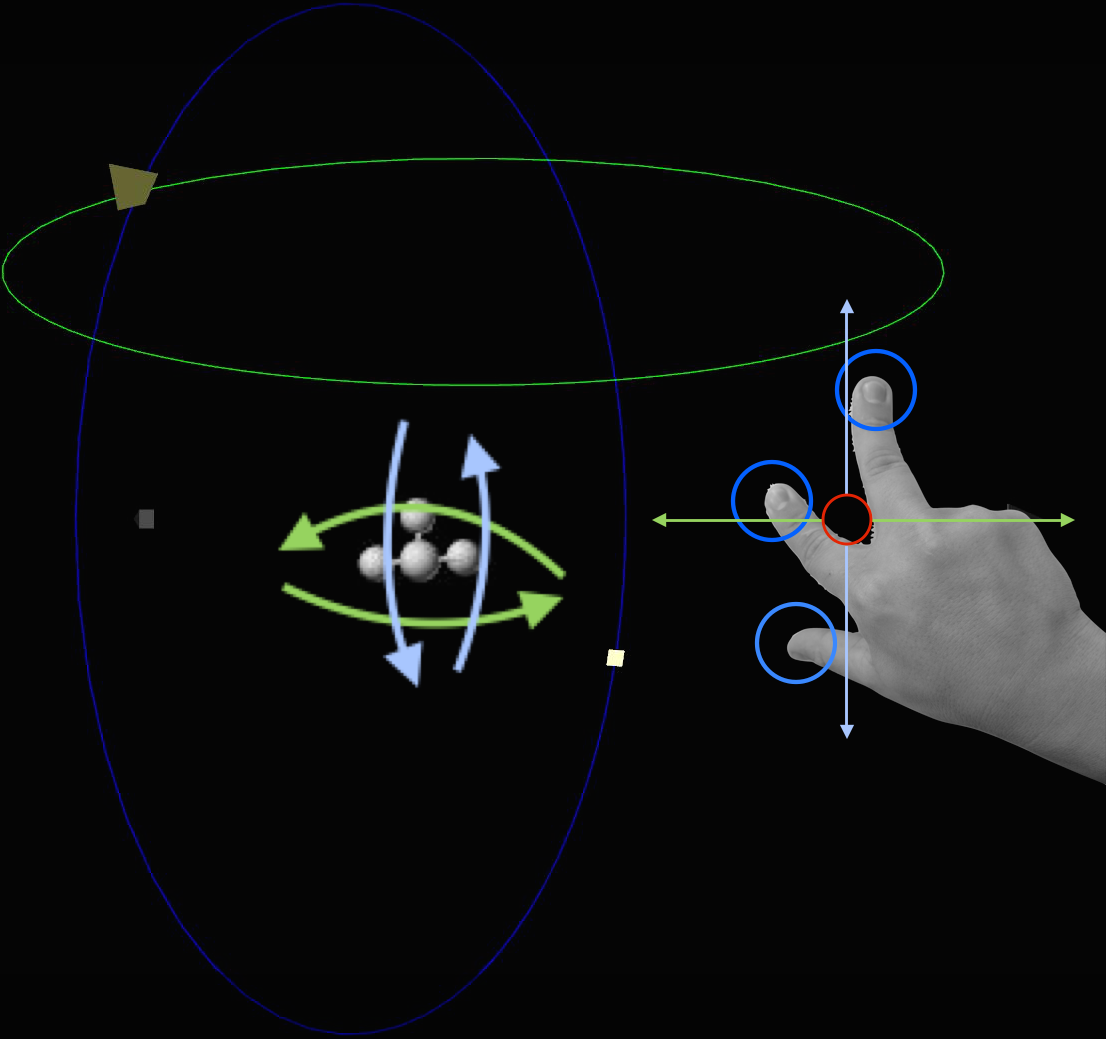
\includegraphics[scale=0.4]{Images/Touch3Fingers.png}
\caption{Three Finger Touch Interaction}
\label{fig: AT3F}
\end{figure}
\end{center}
\subsection {Kinect 2 Camera Gesture implementation}\label{app:KinectGestures}
The Kinect Camera 2.0 has the capability of recognizing the state of the hands. It can differentiate between a closed, open and lasso positions.
See figure \ref{fig: AKHS}.
\begin{center}
\begin{figure}[!h]
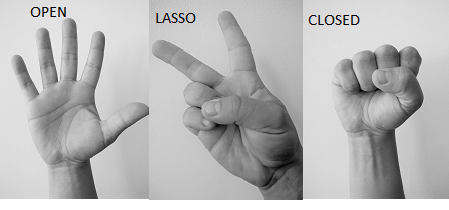
\includegraphics[scale=1.5]{Images/KinectHandStates.png}
\caption{Kinect Hand States}
\label{fig: AKHS}
\end{figure}
\end{center}
Kinect interaction can be activated by holding both hands open for two seconds. For optimal tracking, hands should be away from the body and facing the kinect camera.
See figure \ref{fig: AKI}.
\begin{center}
\begin{figure}[!h]
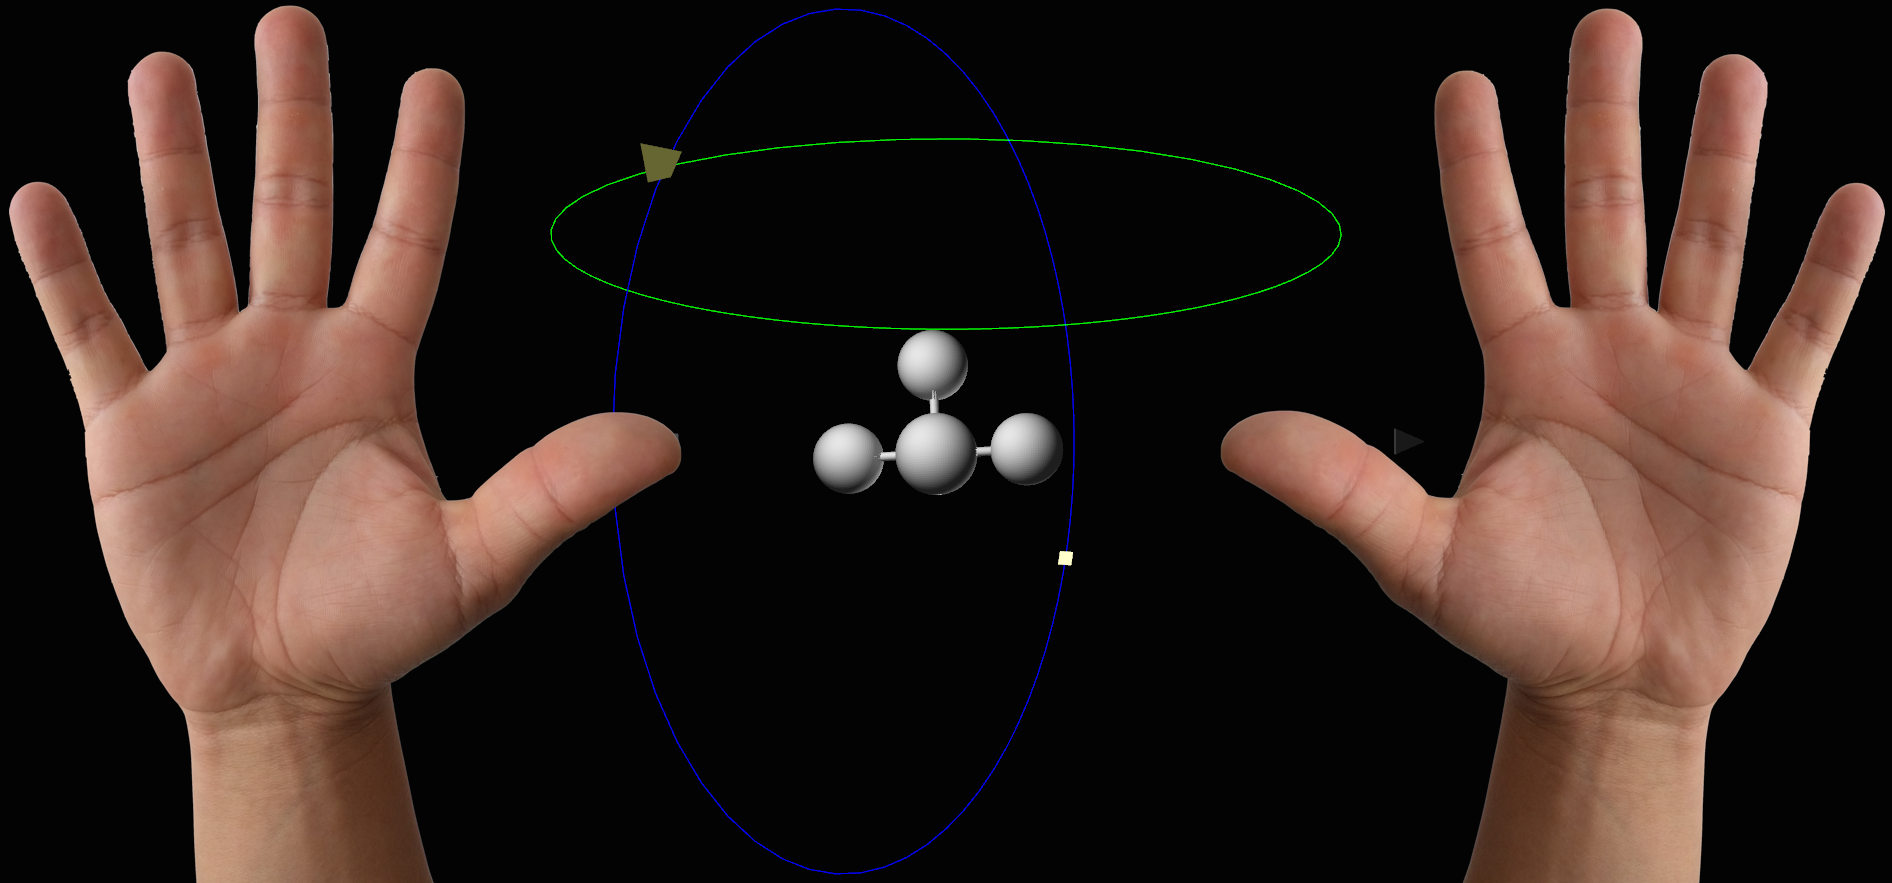
\includegraphics[scale=0.4]{Images/KinectInitialize.png}
\caption{Kinect Initialization Gesture}
\label{fig: AKI}
\end{figure}
\end{center}
Once the interaction is initialized, the following manipulations are possible:
\subsubsection {Rotate}\label{app:subsubsec Rot}
\begin{itemize}
\item Both hands closed start the rotation.\\
\item The object can be rotated in all directions.\\
\item Rotation stops when one hand is opened. \\
\item After this, to restart rotation, open both hands and close them again.\\
\item In this mode the user can also Scale the object. \\
\item The object can be enlarged by separating both hands and shrunk by nearing them.\\
\item Avoid moving both hands on the same direction to reduce object flickering.\\
\item See figure \ref{fig: AKR}.
\end{itemize}
\begin{center}
\begin{figure}[!h]
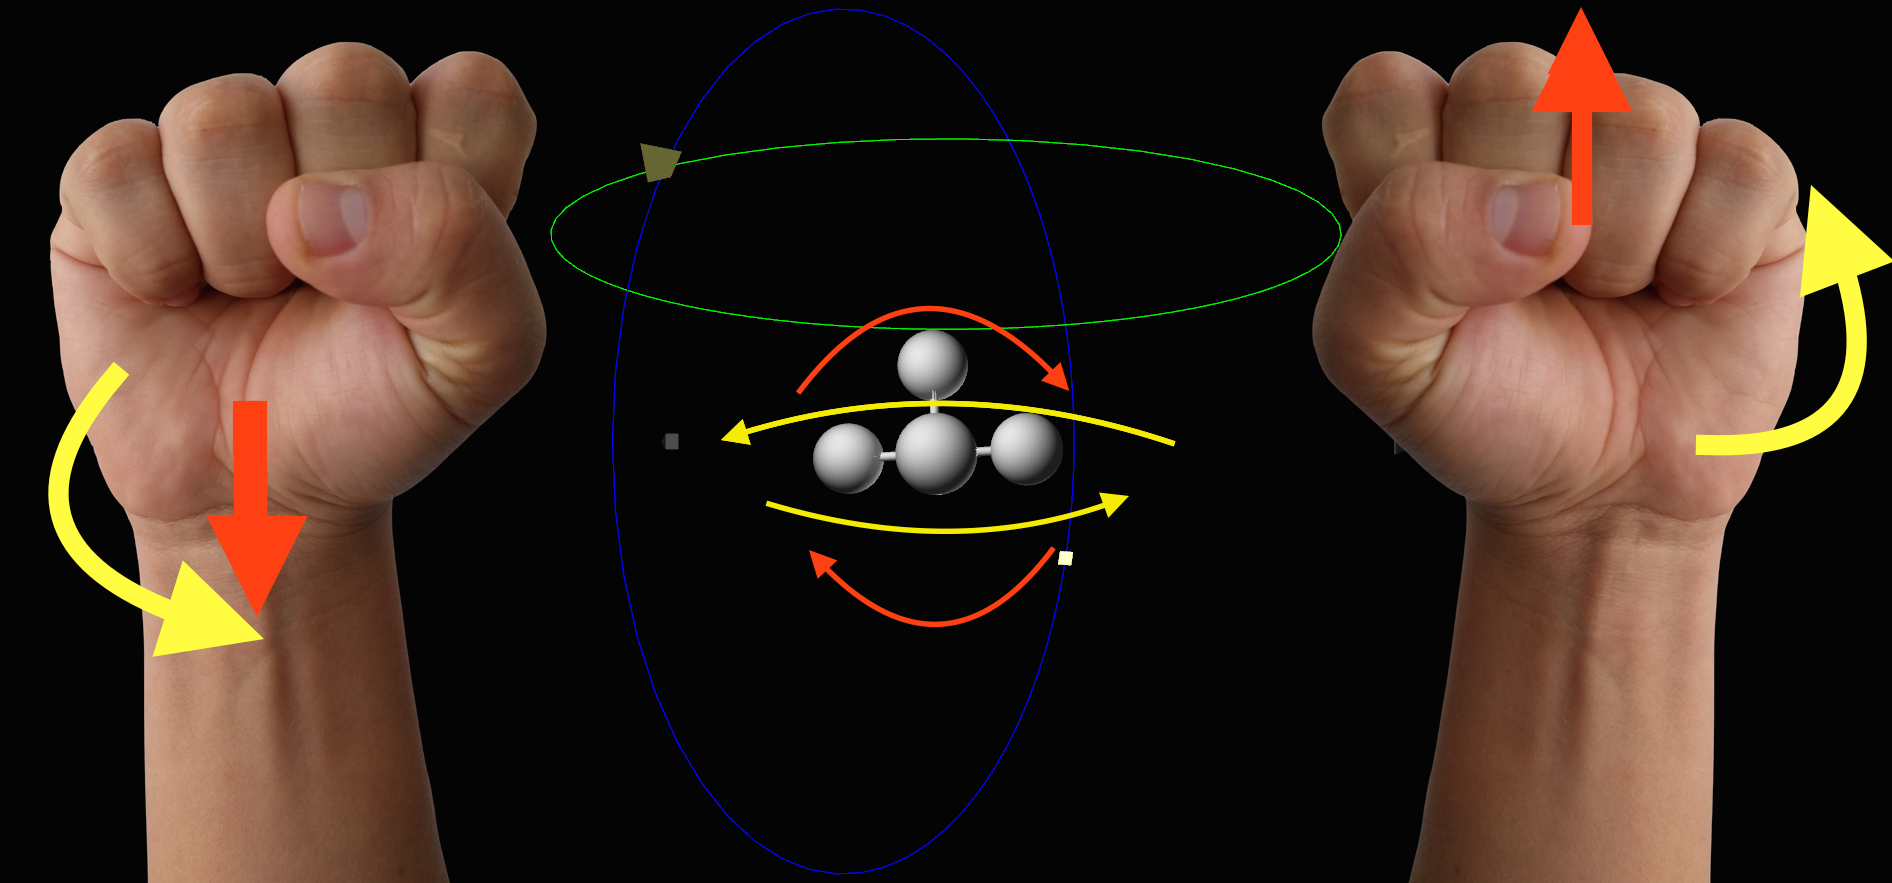
\includegraphics[scale=0.4]{Images/KinectRotate.png}
\caption{Kinect Rotate and Scale}
\label{fig: AKR}
\end{figure}
\end{center}
\subsubsection {Scale}\label{app:subsubsec Scale}
\begin{itemize}
\item Both hands with two fingers up (lasso) initialize the isolated scaling mode. \\
\item The object can be enlarged by separating both hands and shrunk by nearing them.\\
\item See \ref{fig: AKS}.
\end{itemize}
\begin{center}
\begin{figure}[!h]
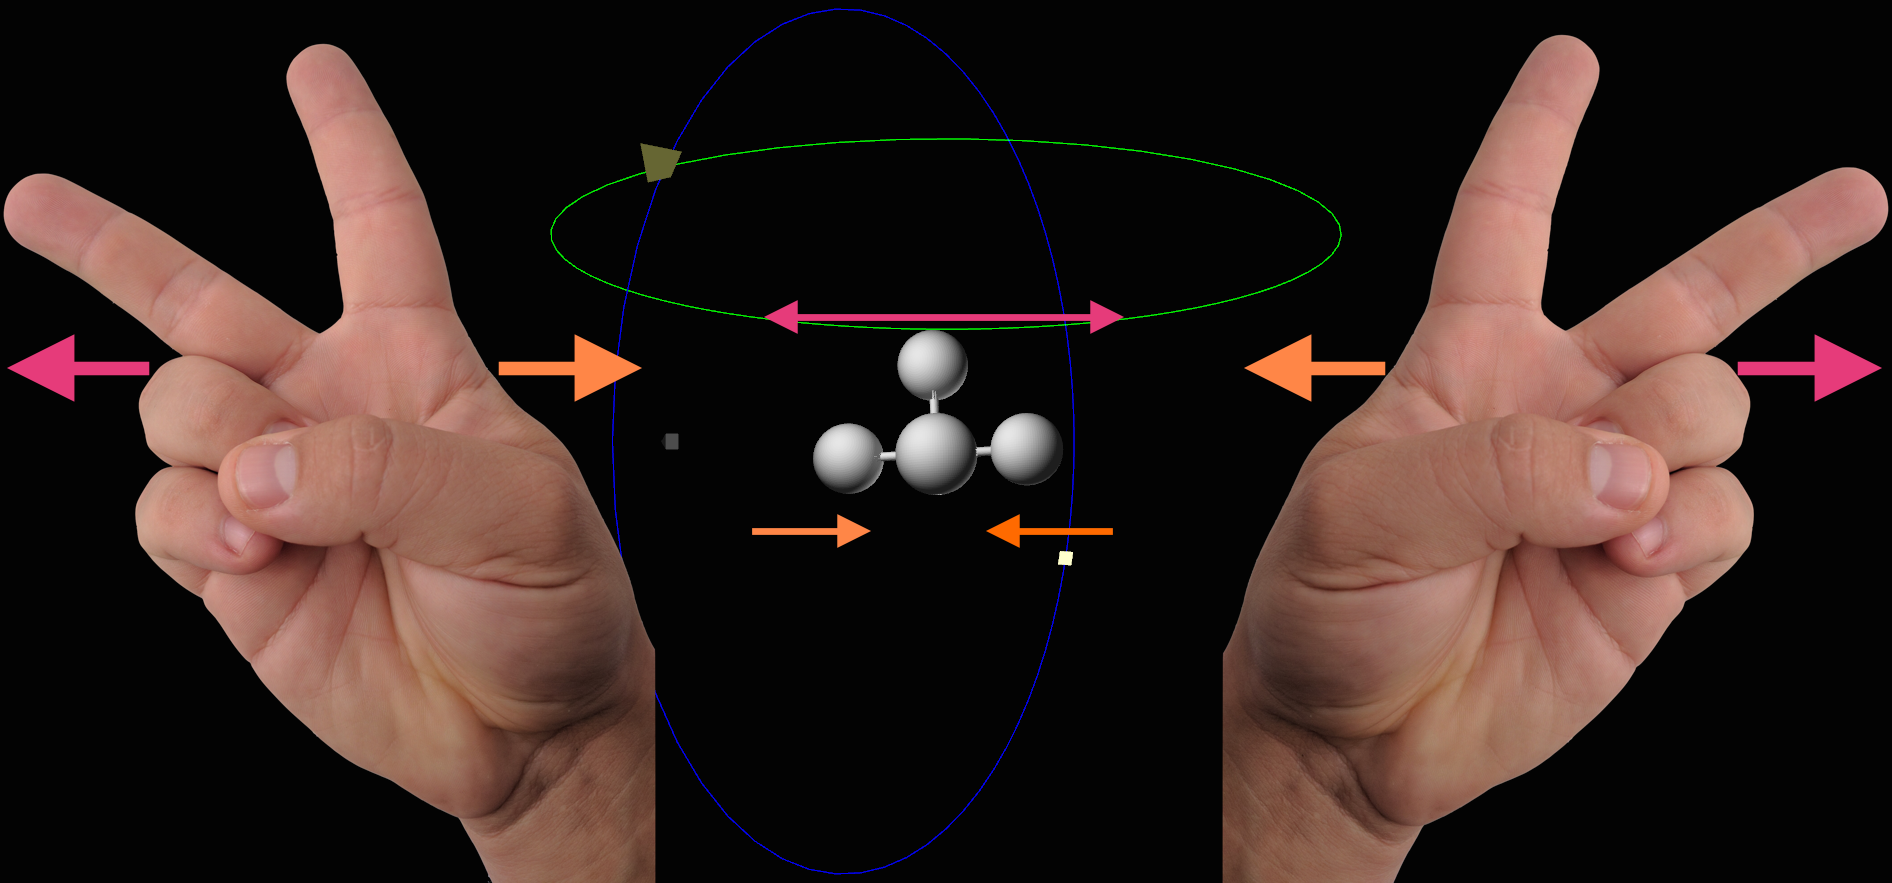
\includegraphics[scale=0.4]{Images/KinectScale.png}
\caption{Kinect Isolated Scale}
\label{fig: AKS}
\end{figure}
\end{center}
\subsubsection {Translate} \label{app:subsubsec Move}
\begin{itemize}
\item The left hand open and the right one closed start the \textbf{object translation}.\\
\item The object follows the movement of the right hand and the left one works as the \lq\lq{}signal\rq\rq{}. \\
\item The movement stays on as long as the left hand remains open, or until the right hand opens.\\
\item See figure \ref{fig: AKMO}.
\end{itemize}
\begin{center}
\begin{figure}[!h]
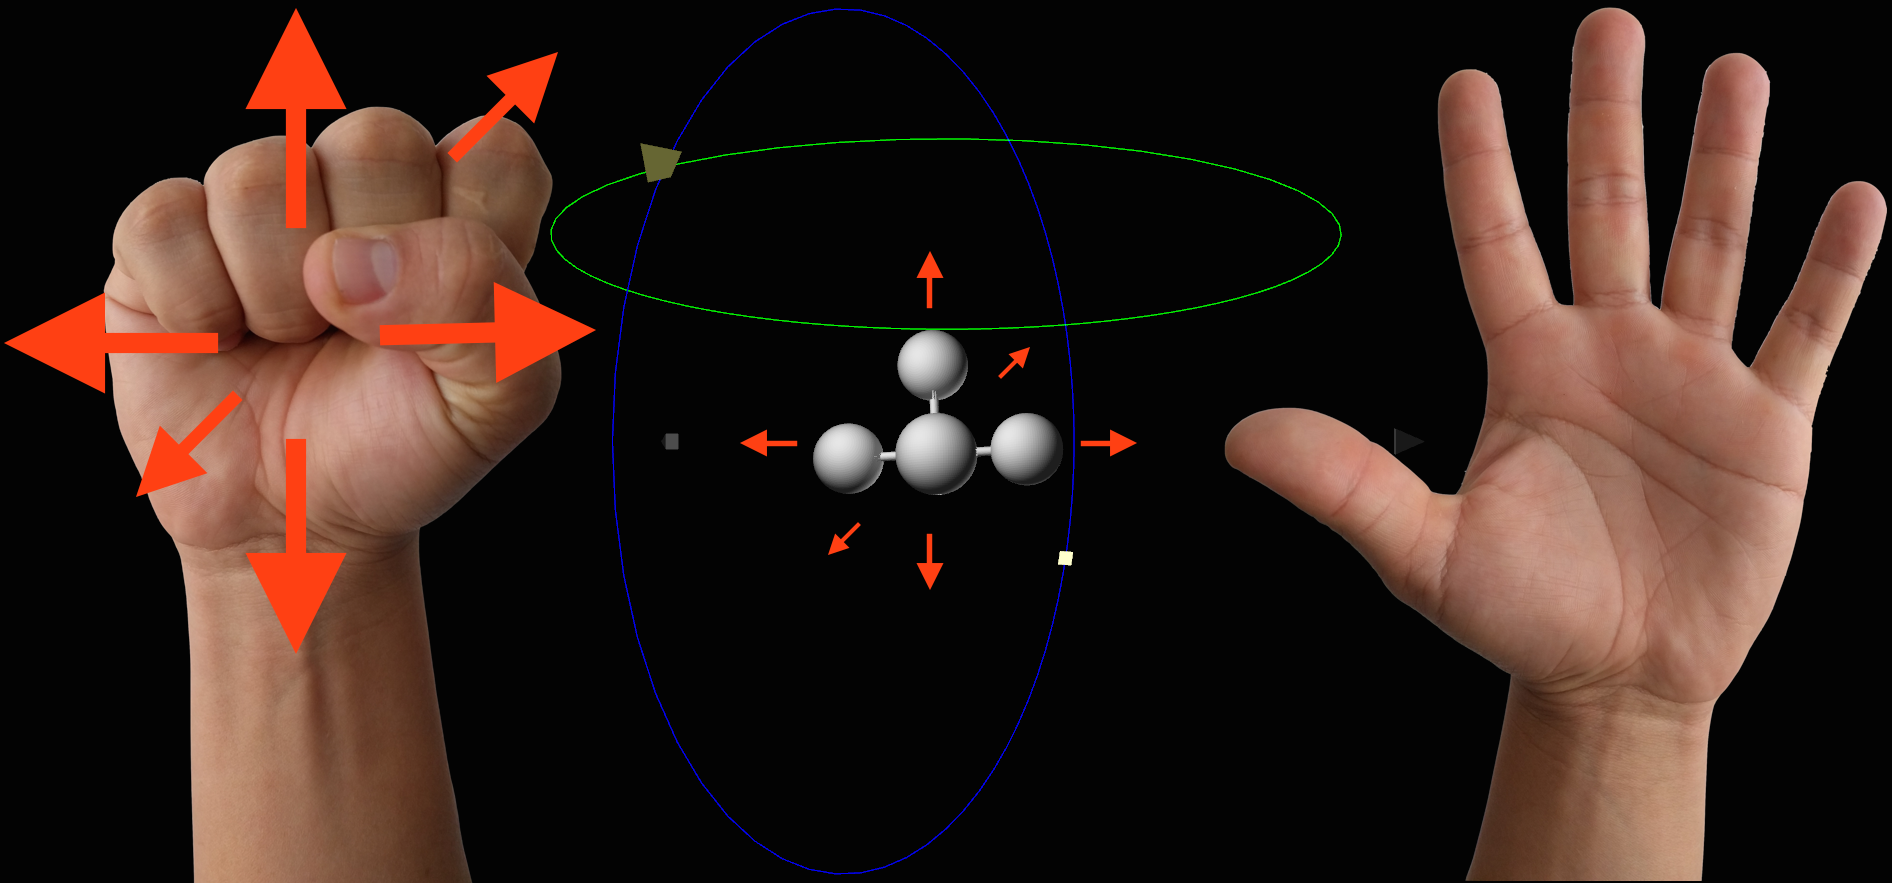
\includegraphics[scale=0.4]{Images/KinectMoveObject.png}
\caption{Kinect Object Translation}
\label{fig: AKMO}
\end{figure}
\end{center}
\begin{itemize}
\item The right hand open and the left one closed start the \textbf{projection translation}.\\
\item The scenario follows the movement of the left hand and the right one works as the \lq\lq{}signal\rq\rq{}.\\
\item The movement stays on as long as the right hand remains open, or until the left hand opens.\\
\item See figure \ref{fig: AKMS}.
\end{itemize}
\begin{center}
\begin{figure}[!h]
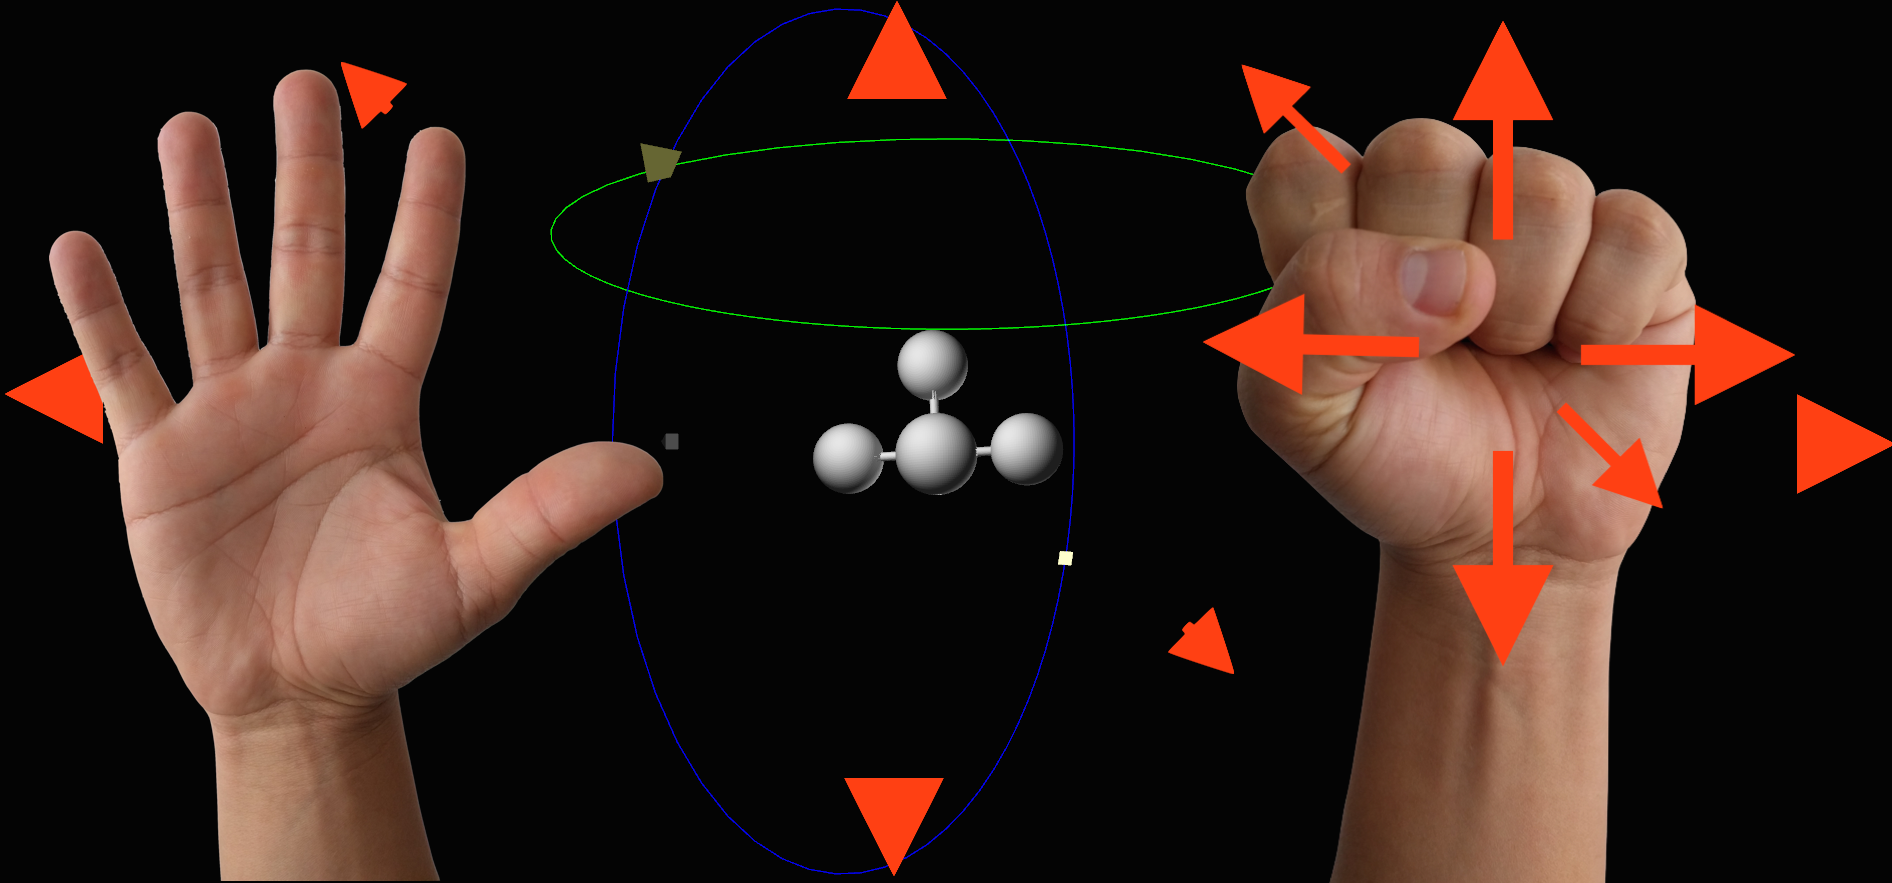
\includegraphics[scale=0.4]{Images/KinectMoveScenario.png}
\caption{Kinect Scenario Translation}
\label{fig: AKMS}
\end{figure}
\end{center}
\subsubsection {Untracked or unknown states} 
If the position of both hands has not been tracked for 5 seconds or if the state of the hand has been unknown for 10 seconds, then the interaction with the kinect camera stops.
\end{appendices}
\end{document}